\documentclass{beamer}
\usetheme{Madrid}
\usepackage[utf8]{inputenc}
\usepackage[ruled,linesnumbered]{algorithm2e}
\usepackage{amsmath,amsthm,amssymb,amsfonts}
\usepackage{mathtools}
\usepackage{booktabs}       % professional-quality tables
\usepackage{graphicx}
\usepackage{array}
\DeclareMathOperator*{\argmin}{argmin}
\DeclareMathOperator*{\argmax}{argmax}

\title[]{Empirical Assessment of HMM and HDP-HSMM Methods}
\subtitle{TTIC 31170 - Robotics}
\author[Lam, Sawhney, Yoo]{A. Lam \and K. Sawhney \and J. Yoo}

\date[June 11, 2019]{June 11, 2019}

\begin{document}

\frame{\titlepage}

\begin{frame}
\frametitle{Outline}
    \begin{enumerate}[I]
        \item Introduction
        \item HMM, HSMM \& HDP-HSMM
        \item Data Generation
        \item Empirical Results
        \item Conclusion
    \end{enumerate}
\end{frame}


\begin{frame}
\frametitle{Introduction - Problem Statement}
    \begin{itemize}
        \item Algorithms to estimate the most likely sequence of hidden states from observations in a \textbf{HMM rely on the Markov assumption} -- that future states are conditionally independent of past states given the present state
        \item The most popular method for estimating these states involves evaluating conditional likelihoods using the forward-backward algorithm, then inferring the most likely sequence of hidden states using the Viterbi algorithm
        \item However, it has been suggested that \textbf{the Markov assumption need not be strictly met} for these techniques to generate reasonably accurate estimates of hidden state sequences
    \end{itemize}
\end{frame}

\begin{frame}
    \frametitle{Introduction - Analysis}
        \begin{itemize}
            \item We sought to \textbf{empirically test this proposition} on the problem of estimating an agent's path in a GridWorld setting
            \item Specifically, we \textbf{simulate agent pathways} under a variety of settings that differ in grid size, placement of obstacles, and transition mechanism, including settings which violate the Markov assumption implicit to traditional HMMs
            \item Hierarchical Dirichlet Process Hidden Semi-Markov Models (\textbf{HDP-HSMMs}) are a Bayesian non-parametric approach to estimating hidden state sequences, where transition, emission and initial state distribution priors are not defined by the user. It is expected that these models will outperform HMMs in non-Markovian settings by better capturing these irregularities
        \end{itemize}
    \end{frame}

\begin{frame}
    \frametitle{HMM \& HSMM}
        A HMM consists of two sequences:
        \begin{itemize}
          \item A \textbf{state sequence} $z = \{z_1, z_2, \dots, z_T\}$ where $z_t$ is the state at timestep $t$ which takes a value from a state space $\mathcal{Z}$ that is assumed to be static and finite for $t = 1, 2, \dots, T$
          \item An \textbf{observation (or emission) sequence} $x = \{x_1, x_2, \dots, x_T\}$ where $x_t$ is the observation at timestep $t$ from an observation space $\mathcal{X}$ that is assumed to be static and finite for $t = 1, 2, \dots, T$
        \end{itemize}

        A HSMM extends a HMM to settings where the sequence of states are \textbf{not strictly Markovian} - instead, the probability of transitioning to a new state $z_{s+1}$ depends on the elapsed time in the current state $z_s$
\end{frame}

\begin{frame}
    \frametitle{Illustration of the HSMM}
    \begin{figure}[H]
    \centering
    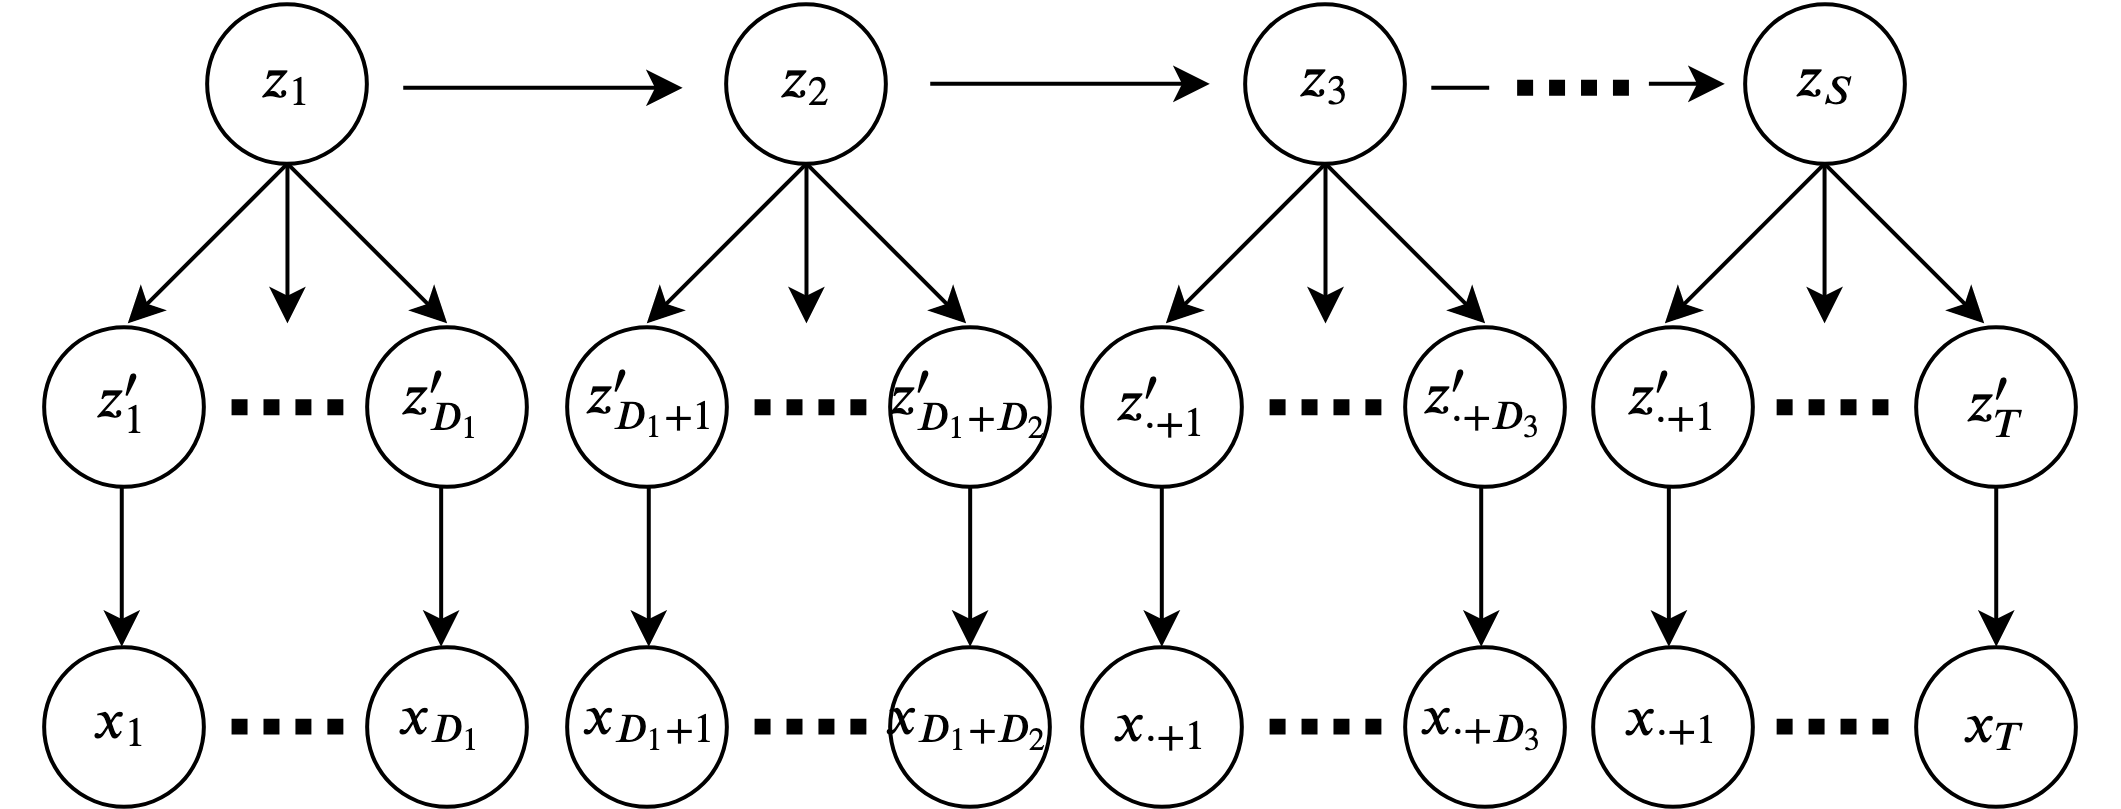
\includegraphics[scale=0.15]{images/hsmm2.png}
    \caption{HSMM where super state transitions are Markovian, while emissions associated with each state follow some explicit duration distribution}
    \label{fig:hsmm}
    \end{figure}
\end{frame}

\begin{frame}
    \frametitle{HDP-HMM}
    A HDP-HMM$(\gamma, \alpha, H)$ model is governed by:
    \begin{itemize}
      \item $\beta_k \coloneqq \beta_k'\cdot \prod_{i=1}^{k-1} (1-\beta_i')$ where $\beta_i' \overset{\text{i.i.d}}{\sim} Beta(1,\gamma)$
      \item $\pi_k \overset{\text{i.i.d}}{\sim} DP(H(\beta), \alpha)$ for $k = 1, \dots, \infty$ where $\beta = \{\beta_k\}_{k=1}^{\infty}$
      \item $z_t \sim \pi_{z_{t-1}}$
      \item $x_t \sim h(\theta_{z_t})$ where $\theta_{k} \sim H$ for $k = 1, \dots, \infty$
    \end{itemize}
    Interpretation:
    \begin{itemize}
        \item $\gamma, \alpha > 0$: concentration parameters, $H$: base distribution of Dirichlet process (DP)
        \item $\{\beta_k\}_{k=1}^{\infty}$: stick-breaking process with parameter $\gamma$
        \item $\{\pi_k \}_{k=1}^{\infty}$: transition distributions drawn from DP, $h(\theta_{z_t})$: observation distributions drawn from $H$
    \end{itemize}
\end{frame}

\begin{frame}
    \frametitle{HDP-HSMM}
    HDP-HSMM is an augmentation of the HDP-HMM to \textbf{include duration distributions}. The main difference is that durations $D_s$ are drawn from base distribution $G$ and sub-states $z'_{t_{s}:t'_{s}}$ are then set to the corresponding super-state $z_{s}$
    \begin{itemize}
      \item $\beta_k \coloneqq \beta_k'\cdot \prod_{i=1}^{k-1} (1-\beta_i')$ where $\beta_i' \overset{\text{i.i.d}}{\sim} Beta(1,\gamma)$
      \item $\pi_k \overset{\text{i.i.d}}{\sim} DP(H(\beta), \alpha)$ for $k = 1, \dots, \infty$ where $\beta = \{\beta_k\}_{k=1}^{\infty}$
      \item $z_s \sim \tilde{\pi}_{z_{s-1}}$
      \item $D_s \sim g(\omega_{z_s})$ where $\omega_k \sim G$ for $k = 1, \dots, \infty$
      \item $z'_{t_{s}:t'_{s}} = z_s$ where $t_{s} = \sum_{s' < s} D_s + 1$ and $t'_{s} = t_{s} + D_s - 1$
      \item $x_{t_{s}: t'_{s}} \overset{\text{i.i.d}}{\sim} h(\theta_{z'_t})$ where $\theta_{k} \sim H$ for $k = 1, \dots, \infty$
    \end{itemize}
\end{frame}

\begin{frame}
    \frametitle{Illustration of HDP-HSMM}
    \begin{figure}[H]
    \centering
    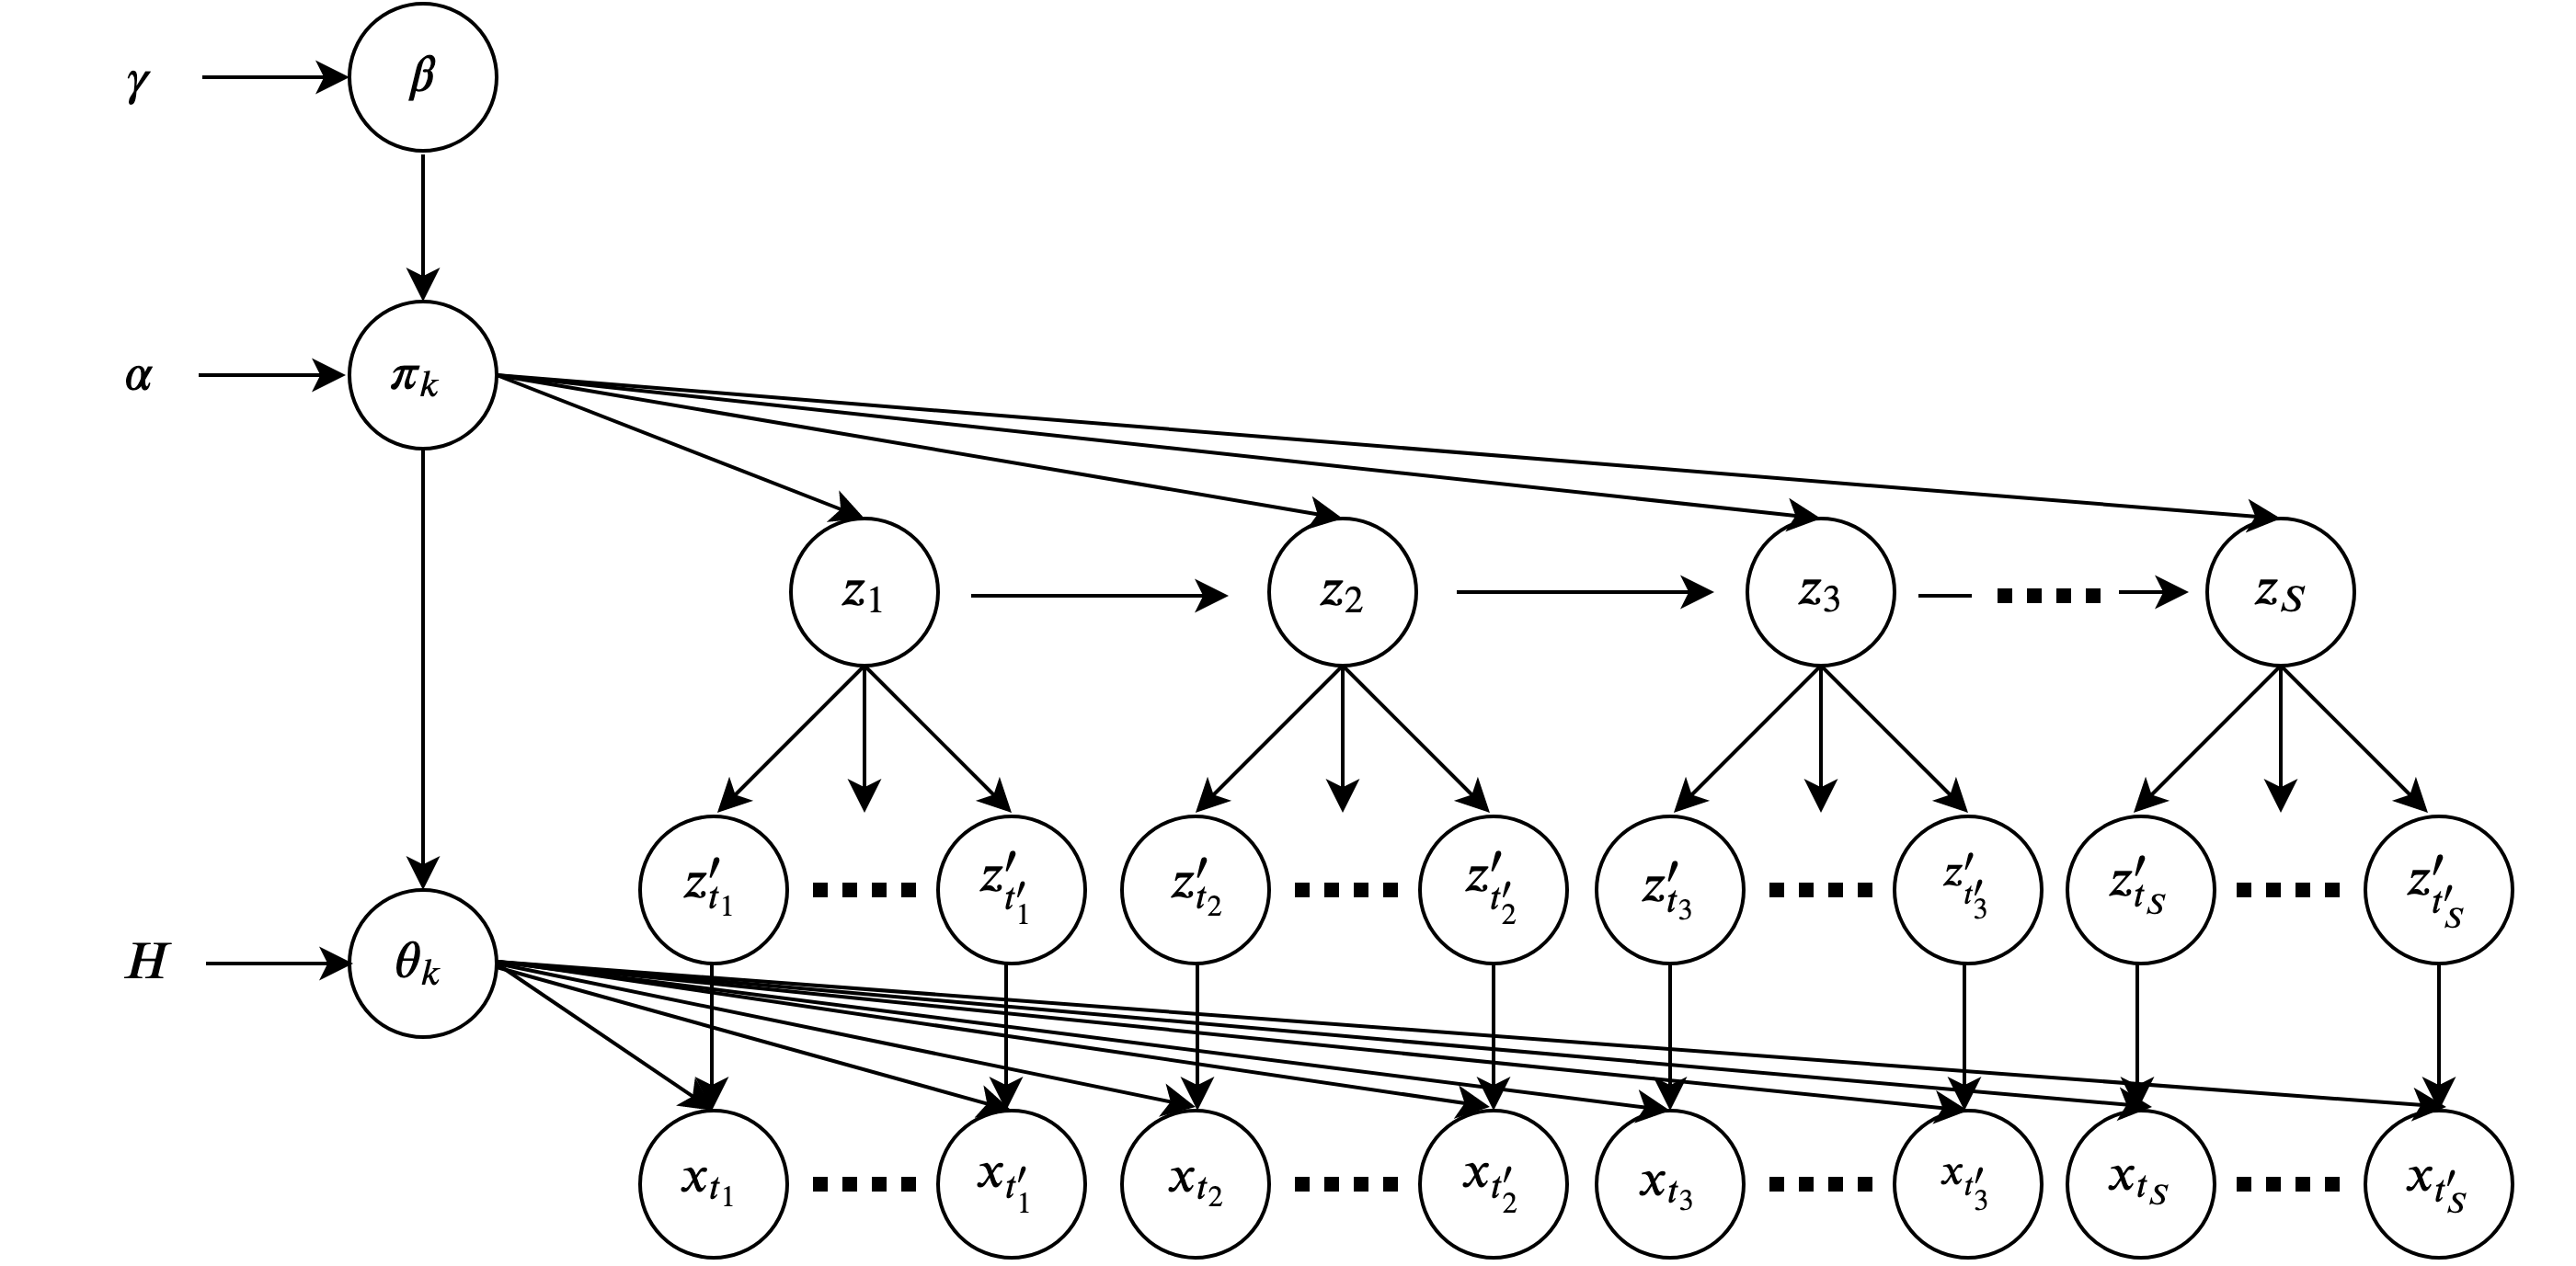
\includegraphics[scale=0.12]{images/hdphsmm.png}
    \caption{HDP-HSMM incorporates a HDP component into a HSMM}
    \label{fig:hdphsmm}
    \end{figure}
\end{frame}

\begin{frame}
    \frametitle{Data Generation - GridWorld Settings}
        \begin{itemize}
            \item \textbf{Grid Size:} 5x5
            \item \textbf{Obstacles:} Different formation of obstacles indicate states that cannot be visited by the agent
        \end{itemize}

        \newcommand{\addmapa}{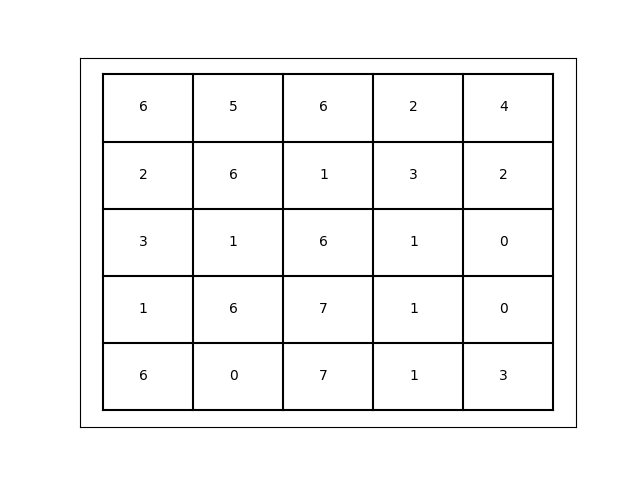
\includegraphics[width=10em]{data/Model1/5x5;4;free.png}}
        \newcommand{\addmapb}{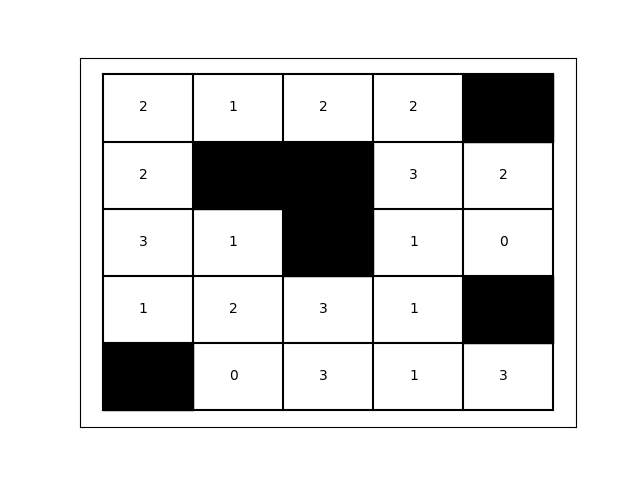
\includegraphics[width=10em]{data/Model2/5x5;4;6box.png}}
        \newcommand{\addmapc}{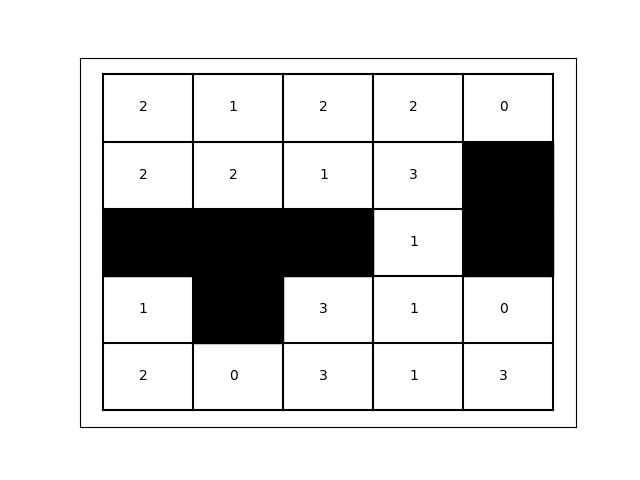
\includegraphics[width=10em]{data/Model3/5x5;4;6sep.png}}
        \newcolumntype{C}{>{\centering\arraybackslash}m{8em}}
        \begin{table}[H]
        \sffamily
        \centering
        \begin{tabular}{l*3{C}@{}}
        \addmapa \addmapb \addmapc \\
        \end{tabular}
        \caption{GridWorld Maps}
        \end{table}
\end{frame}

\begin{frame}
    \frametitle{Data Generation - Agent Motion}
    \begin{itemize}
    \item \textbf{Purely Random}: Uniform transition probability over all states (including current state). This setting satisfies the Markov property, as each realization of a future state is independent from the history of all previous states
    \item \textbf{Traditional Markov}: The state sequences are generated using a fixed transition matrix -- the probability of transitioning from one state to the next is constant as the sequence is generated. This setting also satisfies the Markov property
    \item \textbf{Sticky Transitions}: A sticky process is one where transition probabilities correspond to an agent's elapsed duration in the same state. In our implementation, the probability of staying in the same state decreases geometrically with the duration, and resets upon entering a new state
    \end{itemize}
\end{frame}

\begin{frame}
    \frametitle{Data Generation - Observation Sequences}
    \begin{itemize}
        \item Observations are realizations of a \textbf{Gaussian random variable based on the state}. Each state is randomly assigned a true mean $\mu$, and the standard deviation is identical and fixed at $\sigma = 0.5$ across all states
        \item There are \textbf{eight possible true values of $\mu$}, so some of the 25 states will have the same observation mean
        \item Simulate 10 state sequences of length 200, and observations are then generated using the emission distributions
    \end{itemize}
\end{frame}

\begin{frame}
	\frametitle{Priors for HMM}
	\begin{itemize}
		\item \textbf{Initial State Distribution}: Uniform over all valid states
		\item \textbf{Transition Matrix}: $p = 0.2$ of staying in the same state, remaining probability $p = 0.8$ distributed evenly across valid adjacent states
		\item \textbf{Emission Distribution}: $\mathcal{N}(\mu, \sigma^2)$ based on known true values of $\mu$ and $\sigma$
	\end{itemize}
\end{frame}

\begin{frame}
    \frametitle{Empirical Results}
    \begin{table}[H]
    	\centering
    	\begin{tabular}{|l|l|l|l|}
    		\hline
    		& Map 1 & Map 2 & Map 3 \\
    		\hline
    		Random	& 0.908 & 0.908 & 0.908  \\
    		\hline
    		Markov & 0.483 & 0.435 & 0.440 \\
    		\hline
    		Sticky & 0.460 & 0.475& 0.503 \\
    		\hline
    	\end{tabular}
    	\caption{HMM Results}
    \end{table}

    \begin{table}[H]
    	\centering
    	\begin{tabular}{|l|l|l|l|}
    		\hline
    		& Map 1 & Map 2 & Map 3 \\
    		\hline
    		Random	& 0.908 & N/A  & N/A   \\
    		\hline
    		Markov & 0.768 & 0.758 & 0.765 \\
    		\hline
    		Sticky & 0.790 & 0.788 & 0.785  \\
    		\hline
    	\end{tabular}
    	\caption{HDP-HSMM Results}
    \end{table}
\end{frame}

\begin{frame}
	\frametitle{Discussion - Markov Property in HMM}
	\begin{itemize}
		\item Relaxing the Markov assumptions \textbf{did not lead to significantly worse results}. The reduction in accuracy is small enough to allowapplication of the method to data where the Markov assumption is not met
		\item Having obstacles on the map lowered the misclassification rate in the Markov setting -- obstacles meant having fewer overall hidden states and a \textbf{smaller number of potential paths, which makes the hidden states easier to estimate}
		\item The number of possible true values of $\mu$ had a large effect on the misclassification rate -- \textbf{the more possibilities there were, the better the algorithm performed}
	\end{itemize}
\end{frame}

\begin{frame}
	\frametitle{Discussion - Comparing HMM and HDP-HSMM}
    \begin{itemize}
      \item \textbf{Inferring the number of states}: The HDP-HSMM must correctly infer the true number of states without user-supplied prior information. In our implementation that uses 25 states, this can result in many states being easily mistaken by the HDP-HSMM to be the same state
      \item \textbf{Strength of non-Markovity}: The probability of staying in the same state at any given timestep is $0.2$. Using this level in the sticky motion model tends to only produce weak non-Markovity, and any stickiness to the same state will be ephemeral compared to settings where the probability level is larger
      \item \textbf{Convergence}: There is some concern about whether the HDP-HSMM converged sufficiently in our experiments. Tests with longer sequences and more sequences did not yield significantly different results, but it is not clear what scale is appropriate given the problem space
    \end{itemize}
\end{frame}

\begin{frame}
    \frametitle{Discussion - HDP-HSMM Diagnostics}
    \newcommand{\addrandommeana}{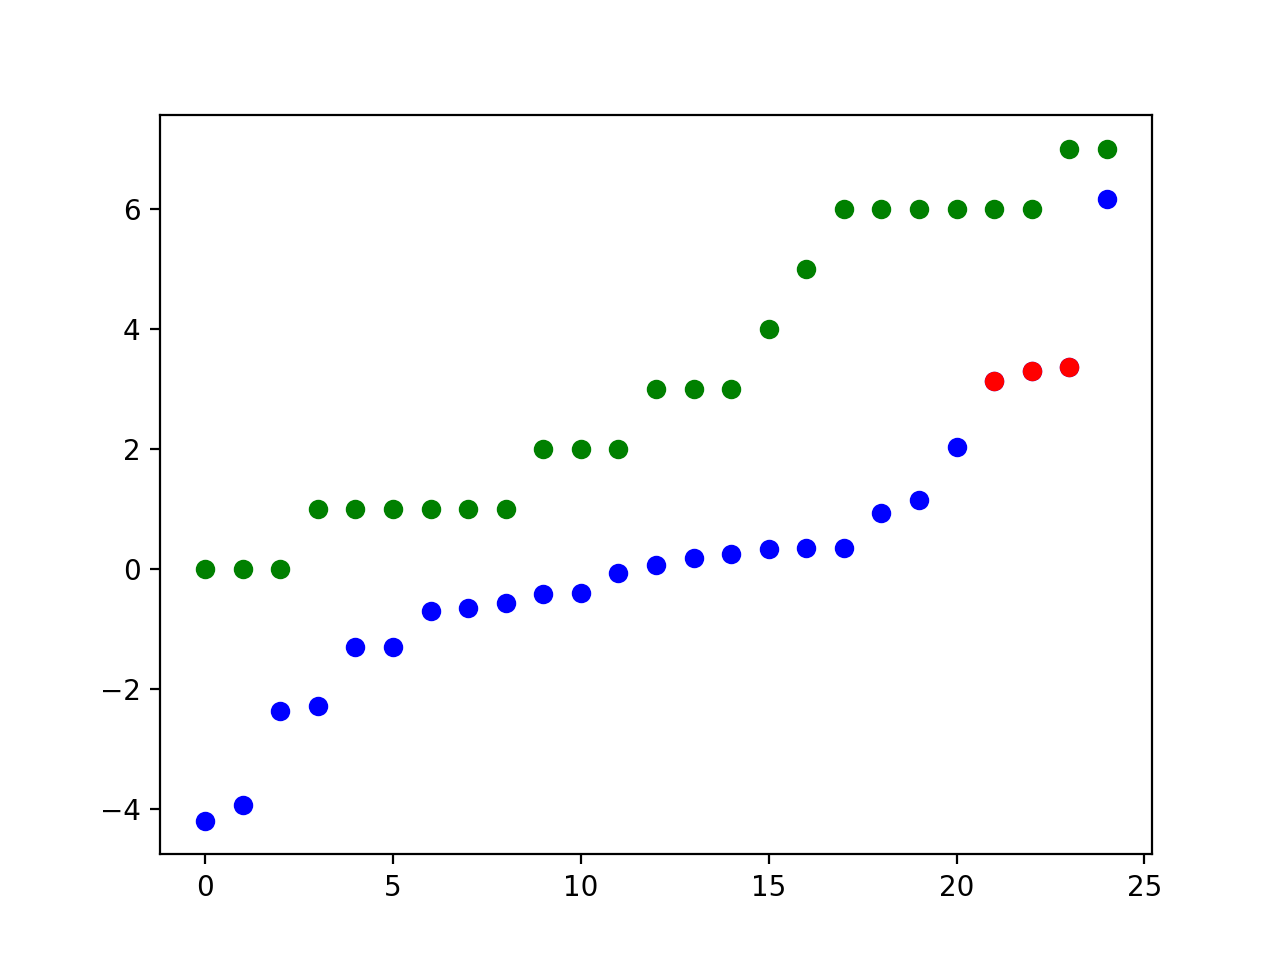
\includegraphics[width=10em]{images/hdphsmm/random-m1-means.png}}
    \newcommand{\addmarkovmeana}{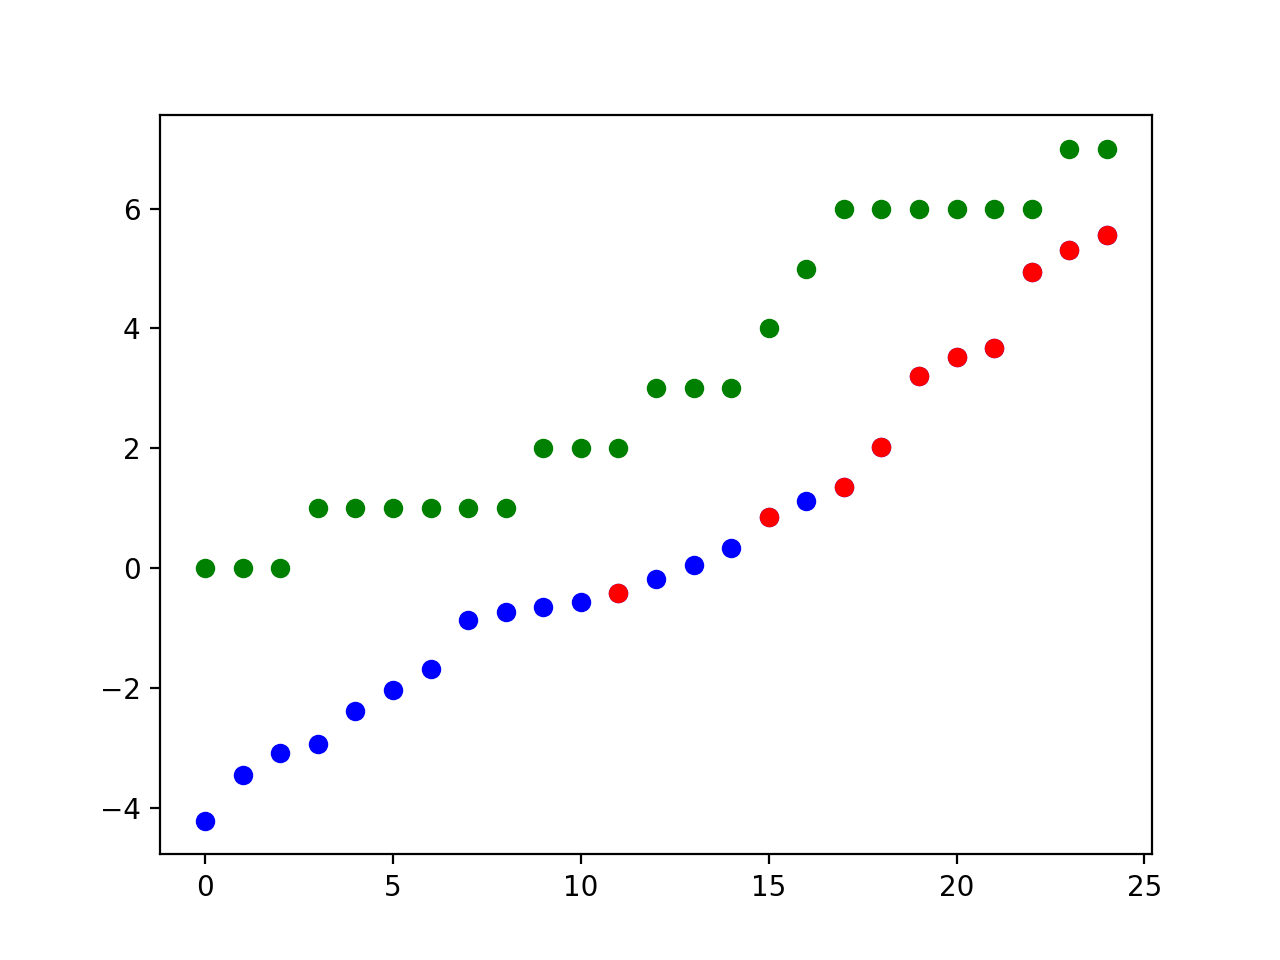
\includegraphics[width=10em]{images/hdphsmm/markov-m1-means.png}}
    \newcommand{\addcorrmeana}{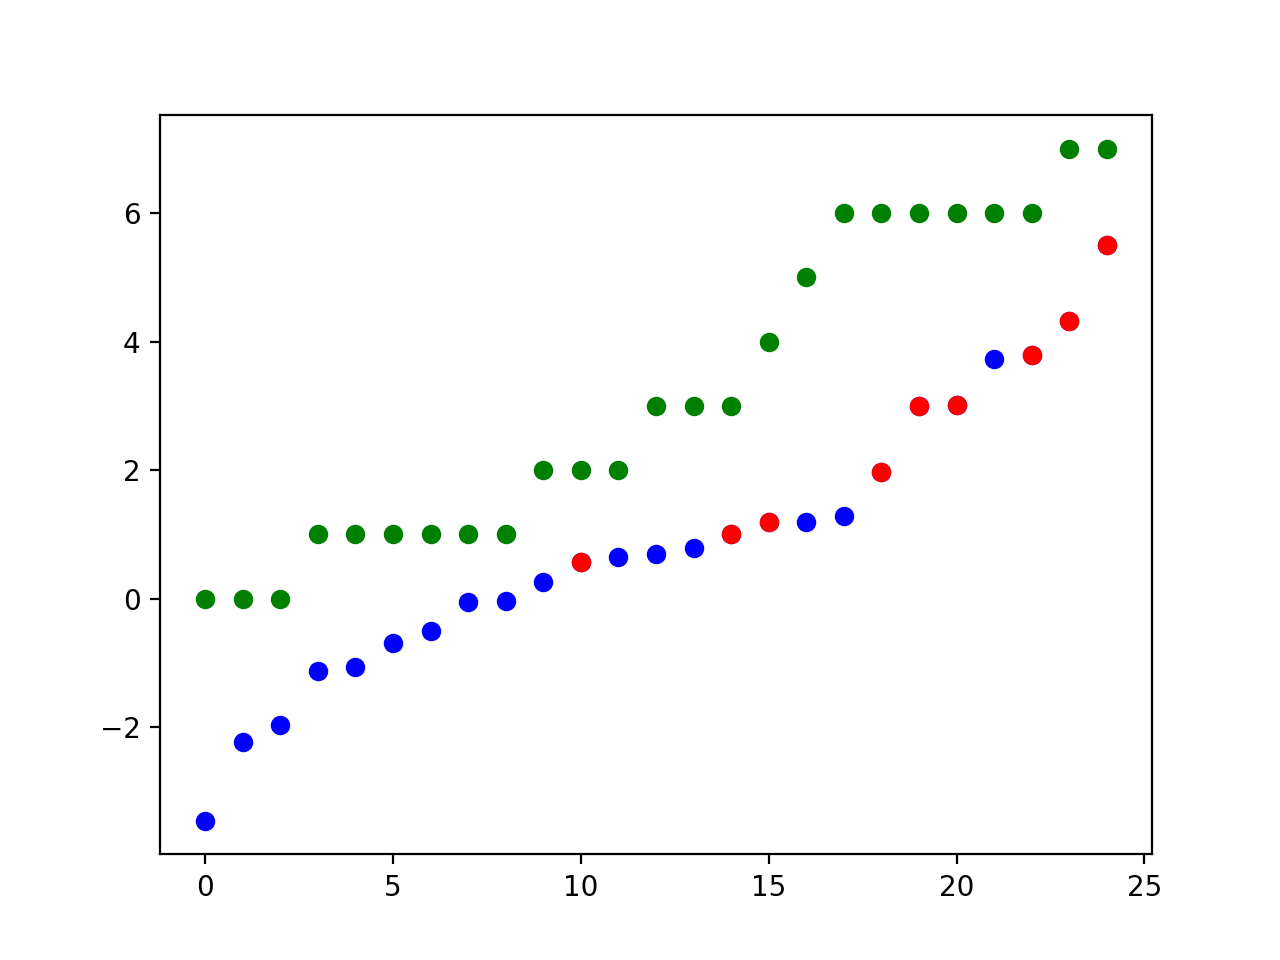
\includegraphics[width=10em]{images/hdphsmm/corr-m1-means.png}}
    \begin{table}[H]
	    \sffamily
	    \centering
	    \begin{tabular}{l*4{c}@{}}
	    \addrandommeana \addmarkovmeana \addcorrmeana \\
	    \end{tabular}
	    \caption{Estimated means and true means for different motions (random, Markov and sticky) through Map 1}
	    \label{table:meaninfer}
    \end{table}
\end{frame}

\begin{frame}
    \frametitle{Discussion - HDP-HSMM Diagnostics}
    \newcommand{\addrandomseqa}{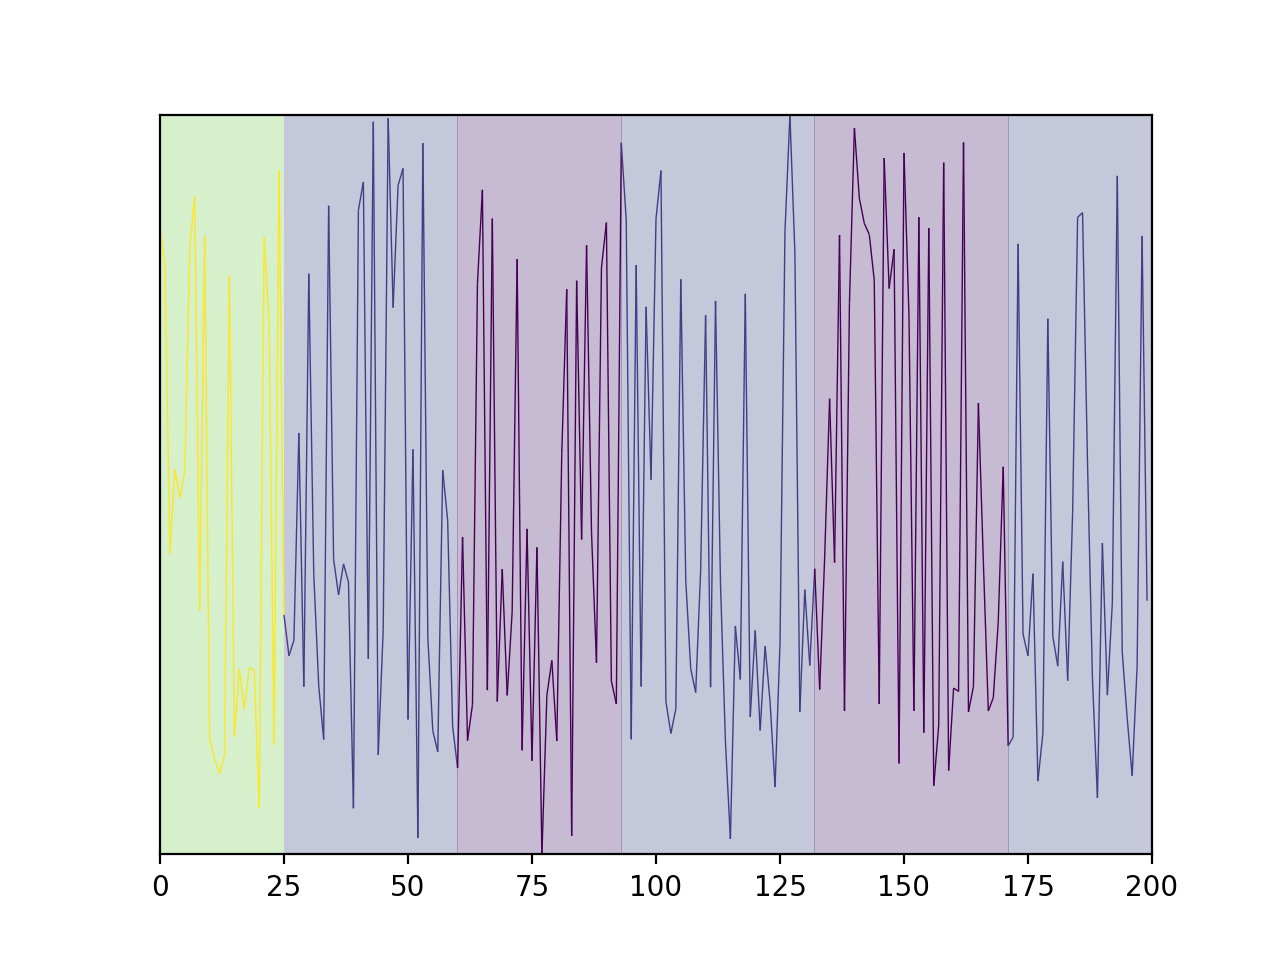
\includegraphics[width=10em]{images/hdphsmm/random-m1-seq.png}}
    \newcommand{\addmarkovseqa}{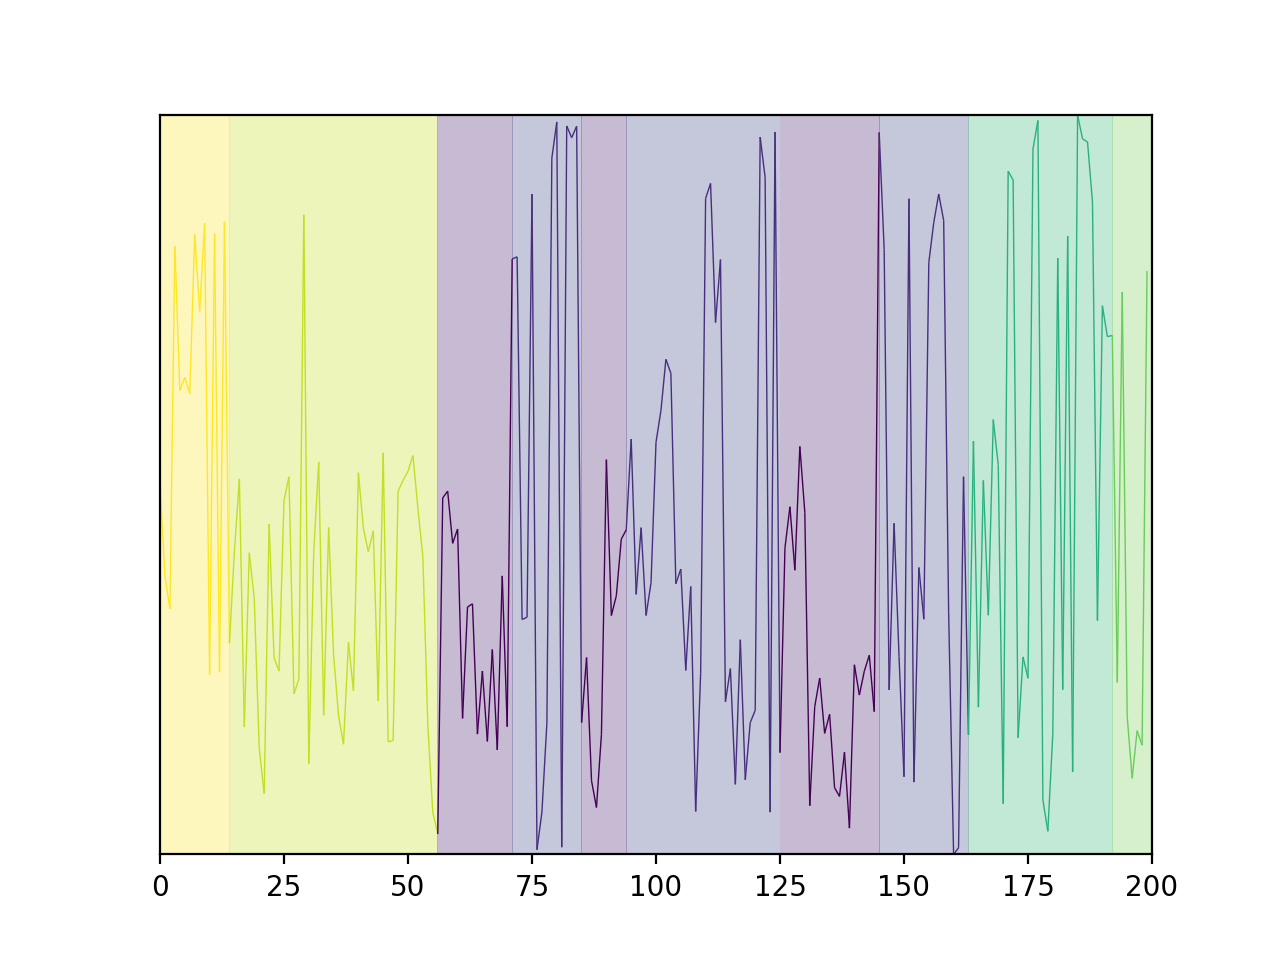
\includegraphics[width=10em]{images/hdphsmm/markov-m1-seq.png}}
    \newcommand{\addcorrseqa}{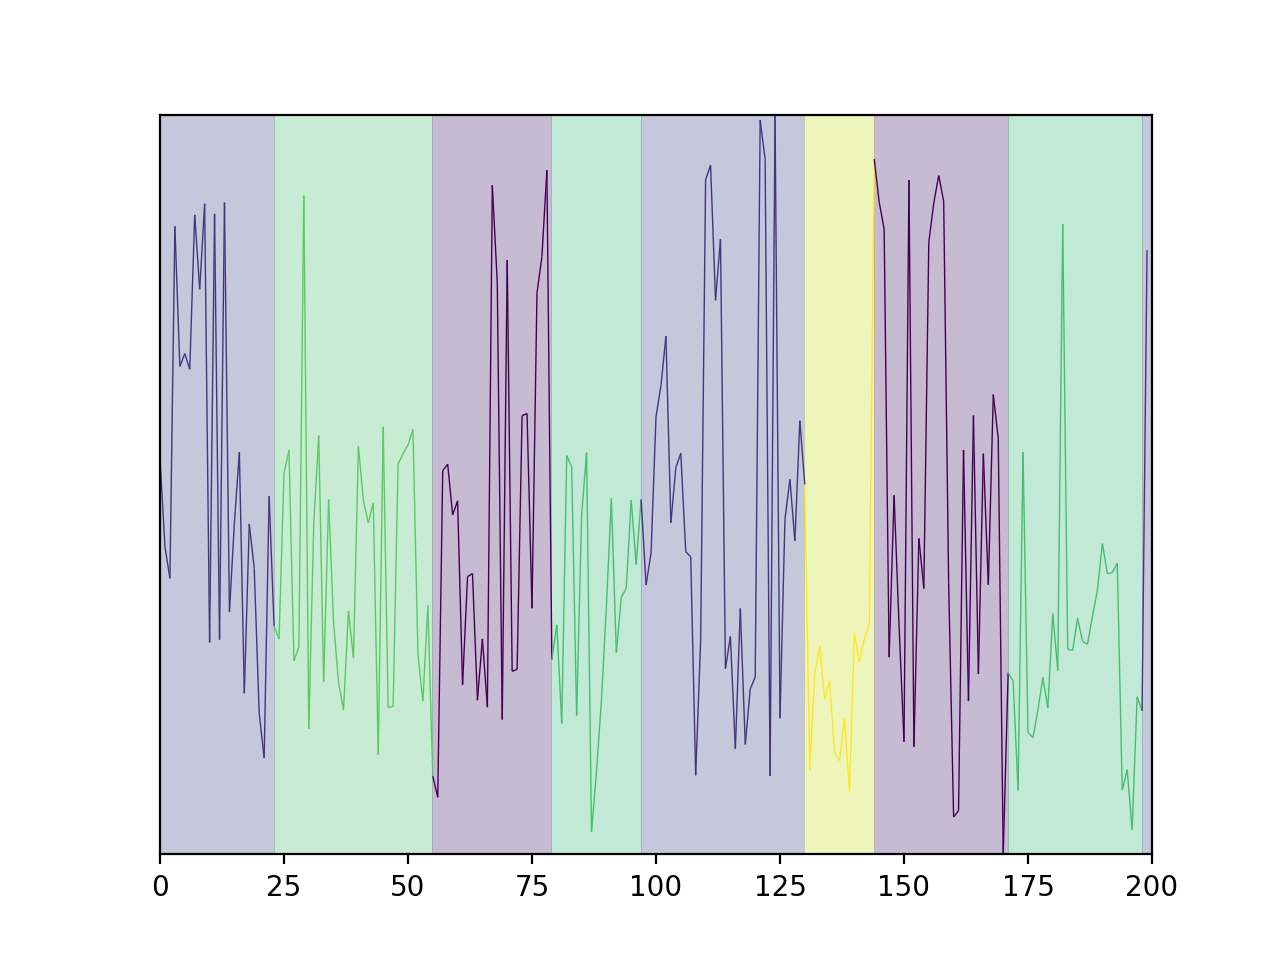
\includegraphics[width=10em]{images/hdphsmm/corr-m1-seq.png}}
    \begin{table}[H]
    \sffamily
    \centering
    \begin{tabular}{l*4{c}@{}}
    \addrandomseqa \addmarkovseqa \addcorrseqa \\
    \end{tabular}
    \caption{Observation sequences mapped to inferred states for different motions (random, Markov and sticky) through Map 1}
    \label{table:stateinfer}
    \end{table}
\end{frame}



\begin{frame}
	\frametitle{Conclusions}
	\begin{itemize}
		\item \textbf{HMM Performance in Non-Markov Settings}: The classic HMM method produced reasonable results even when applied to data that violates the Markov assumption.
		\item \textbf{Accuracy of HMM vs. HDP-HSMM}: In our test settings, the HMM method had a much lower misclassification rate than the HDP-HSMM method. We set up the HMM with a well-informed prior, while the HDP-HSMM method struggled to infer the correct number of states.
	\end{itemize}
\end{frame}

\begin{frame}
	\frametitle{Future Work}
		\begin{itemize}
			\item Expand our experiments through generating more data, including using different random generator seeds, different grid sizes and obstacle placements, and adjusting the transition and emission distributions.
			\item Test the accuracy of the HMM under less-informative priors.
			\item We could strengthen the non-Markovity and make the true means of the states more distinct, to see how the HDP-HSMM performs in that setting.
		\end{itemize}
\end{frame}

\begin{frame}
	\centering
	\huge{Questions?}
\end{frame}


\begin{frame}
    \frametitle{References}
    \begin{itemize}
        \item [1] Johnson, M.J.\ \& Willsky, A.S.\ (2013) Bayesian Nonparametric Hidden Semi-Markov Models, {\it Journal of Machine Learning Research 14 (2013)},
        pp.\ 673--701. Cambridge, MA: MIT Press.
    \end{itemize}
\end{frame}

\end{document}
